\begin{activity} \label{A:6.4.2}  In each of the following problems, determine the total work required to accomplish the described task.  In parts (b) and (c), a key step is to find a formula for a function that describes the curve that forms the side boundary of the tank.
\begin{figure}[h]
\begin{center}
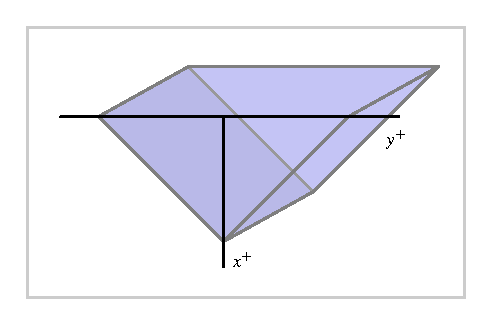
\includegraphics{figures/6_4_Act2Trough.eps}
\caption{A trough with triangular ends, as described in Activity~\ref{A:6.4.2}, part (c).} \label{F:6.4.Act2Trough}
\end{center}
\end{figure}
\ba
	\item Consider a vertical cylindrical tank of radius 2 meters and depth 6 meters.  Suppose the tank is filled with 4 meters of water of mass density 1000 kg/m$^3$, and the top 1 meter of water is pumped over the top of the tank.
	\item Consider a hemispherical tank with a radius of 10 feet.  Suppose that the tank is full to a depth of 7 feet with water of weight density 62.4 pounds/ft$^3$, and the top 5 feet of water are pumped out of the tank to a tanker truck whose height is 5 feet above the top of the tank.
	\item Consider a trough with triangular ends, as pictured in Figure~\ref{F:6.4.Act2Trough}, where the tank is 10 feet long, the top is 5 feet wide, and the tank is 4 feet deep.  Say that the trough is full to within 1 foot of the top with water of weight density 62.4 pounds/ft$^3$, and a pump is used to empty the tank until the water remaining in the tank is 1 foot deep.
\ea

\end{activity}
\begin{smallhint}
\ba
	\item Small hints for each of the prompts above.
\ea
\end{smallhint}
\begin{bighint}
\ba
	\item Big hints for each of the prompts above.
\ea
\end{bighint}
\begin{activitySolution}
\ba
	\item Solutions for each of the prompts above.
\ea
\end{activitySolution}
\aftera